\documentclass{article}
% \documentclass{beamer}
% \usetheme{Madrid}

%------------------------------
% used to include other .tex files
\usepackage{standalone}

% for symbols like degree
\usepackage{gensymb}  

% used for href/url
\usepackage{hyperref}


% used for math fomulas
\usepackage{amsmath}

% used for pictures
\usepackage{graphicx}
\usepackage{subcaption}
\usepackage{float}

% used for codes
\usepackage{listings}
\lstset{
  basicstyle=\ttfamily\footnotesize, % Set your code to be drawn with a monospaced font
  breaklines=true, % Enables line breaking
  frame=single % Adds a frame around the code
}

% used for Graph
\usepackage{adigraph}

% used for Bayesian Network
\usepackage{tikz}
\usetikzlibrary{bayesnet}

%------------------------------
% TODO 
\tolerance=10000
\emergencystretch=\maxdimen
\hyphenpenalty=10000
\hbadness=10000


\usepackage{silence}
\WarningFilter{latex}{Overfull \hbox}

%------------------------------



\title{MK's Notes for CIVL-4530 Geometric Design}
\date{2024-03-04}
\author{Michael Chen}

\begin{document}
  \pagenumbering{gobble}
  \maketitle

  \begin{align*}
  & \textbf{TODO: make the page number consistent}
  \\
  \\
  \\
  \\
  \\
  \\
  \\
  \\
  & \text{Geometric design is the base of transportation,}\\ 
  \\
  & \text{providing fundamental concepts, terms, and fomulas.}\\
  \end{align*}
  \newpage
  \pagenumbering{arabic}
  % \setcounter{page}{0}

  % todo ----------------------------------------
  \tableofcontents
  \newpage


  % include all chapters
  \documentclass{article}
% \documentclass{beamer}
% \usetheme{Madrid}

%------------------------------
% used for href/url
\usepackage{hyperref}


% used for math fomulas
\usepackage{amsmath}

% used for pictures
\usepackage{graphicx}
\usepackage{subcaption}
\usepackage{float}

% used for codes
\usepackage{listings}
\lstset{
  basicstyle=\ttfamily\footnotesize, % Set your code to be drawn with a monospaced font
  breaklines=true, % Enables line breaking
  frame=single % Adds a frame around the code
}

% used for Graph
\usepackage{adigraph}

% used for Bayesian Network
\usepackage{tikz}
\usetikzlibrary{bayesnet}

%------------------------------
% TODO 
\tolerance=10000
\emergencystretch=\maxdimen
\hyphenpenalty=10000
\hbadness=10000


\usepackage{silence}
\WarningFilter{latex}{Overfull \hbox}

%------------------------------



\title{MK's Notes for CIVL-4530 Geometric Design}
\date{2024-03-04}
\author{Michael Chen}

\begin{document}
  \pagenumbering{gobble}
  \maketitle
  \newpage
  \pagenumbering{roman}


  % ----------------------------------------
  \tableofcontents
  \newpage


  % ----------------------------------------
  Geometric Design is a basic course of Transportation, introducing principal concepts and fomulas.

  \newpage

  % ----------------------------------------
  \setcounter{section}{0}
  \section{Chapter 01 Introduction and Highway Function}
  \subsection{Objectives}
  \begin{enumerate}
    \item Geometric Design concepts
    \item Highway Funciton
  \end{enumerate}

  \subsection{Geometric Design Definition}
  \begin{enumerate}
    \item fit the highway to the terrain
    \item maintaining design standards for safety and performance
  \end{enumerate}

  \subsection{Geometric Design Basic}
  \begin{enumerate}
    \item make criteria matches  
    \begin{enumerate}
      \item driver expectancy/behavior
      \item vehicle performance/behavior
    \end{enumerate}
    \item balance safty, cost, mobility, community values, environmental, politics, liability, sustainable development, etc
  \end{enumerate}

  \subsection{AASHTO Role}
  \begin{enumerate}
    \item American Association of State Highway and Transportation Officials
    \item the membership of AASHTO consists of FHWA, and state DOTs
  \end{enumerate}

  % ----------------------------------------
  \subsection{Reference - AASHTO publications}
  \begin{enumerate}
    \item \textbf{a.k.a Green Book/PGDHS:} A Policy on Geometric Design of Highways and Streets, 2018, 7th Edition
    \item Guidelines for Geometric Design of Very Low Volume Local Roads, 2001
    \item A Guide to Achieving Flexibility in Highway Design, May 2004
    \item Guide for the Planning, Design, and Operation of Pedestrian Facilities, July 2004
    \item Guide for the Development of Bicycle Facilities, June 2012

    \item Good for New Highway Design 
    \item TRB Special Report 214, Designing Safer Roads: Practices for Resurfacing, Restoration, and Rehabilitation for guidance. \\
  \end{enumerate}

  \subsection{Reference - ITE publications}
  \begin{enumerate}
    \item Urban Street Geometric Design Handbook, 2008
    \item Freeway and Interchange Geometric Design Handbook, 2007
    \item Designing Walkable Urban Thoroughfares: A Context Sensitive Approach, March 2010
  \end{enumerate}

  % ------------------ todo

  \subsection{Older Driver Deficiencies}


  \begin{tabular}{|c|c|c|c|c|}
    Roadway & urban & rural level & rural rolling & rural mountainous\\
    \hline
    Freeway & C/D   & B & B & C\\
    Arterial & C/D  & B & B & C\\
    Collector & D   & C & C & D\\
    Local & D       & D & D & D\\
  \end{tabular}
  \begin{figure}[h!]
    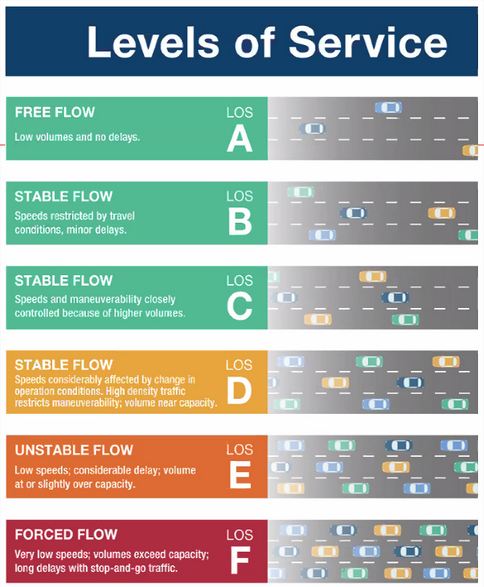
\includegraphics[width=\linewidth]{LOS.png}
    \caption{Level of Service}
    \label{fig:image-LOS}
  \end{figure}

  \subsection{13 AASHTO Criteria}
  \begin{enumerate}
      \item design speed
      \item lane width
      \item shoulder width
      \item bridge width
      \item structural capacity
      \item 
      \item horizontal alignment
      \item vertical alignment
      \item cross slope
      \item grades
      \item superelevation
      \item horizontal clearance
      \item vertical clearance
  \end{enumerate}

  \subsection{speed}
  \begin{enumerate}
    \item running speed - the speed of an individual vehicle
    \item design speed - AASHTO: max safe speed
    \item operation speed - the 85th percentile of observed speed in free flow conditions
    \item safty of over speed - $\Delta$V: [0, 5] low; [5, 15] medium; [15, infinit] high
  \end{enumerate}

  minimum design speed for \textbf{rural} roadways vs vehicle per day(VPD)
  \begin{tabular}{|c|c|c|c|}
    \hline
    rural terrain & 0-400 & 400-2000 & over 2000 \\
    \hline
    level         & 40    & 50       & 60 \\
    rolling       & 30    & 40       & 50 \\
    mountainous   & 20    & 30       & 40 \\
  \end{tabular}

  \subsection{lane width for urban and rural (1-2ft wider than urban)}
  \begin{tabular}{|l|l|l|}
    Types & urban & rural \\
    \hline
    Freeway and Interstates: & 12ft, & 12ft\\
    Ramp: & 12-30ft & 12-30ft \\ 
    Arterial: & 11-12ft, & 10-12ft \\
    Collections: & 10-12ft, & 10-12ft\\
    local roads: & 9-12ft, & 9-12ft  \\
  \end{tabular}

  \subsection{cross slope}
  paved surfaces: 1.5-2\%, typical 2\%  - Green Book\\
  unpaved surfaces: 2-6\% - Green Book\\
  areas with high intensity rainfall: 2-2.5\% \\
  ALDOT use in 2 Counties: 2.2\% \\



\begin{table}[ht]
\centering
\caption{Lane Widths for Different Types of Roadways}
\label{tab:lane_widths}
\begin{tabular}{@{}lcccc@{}}
\hline
\textbf{Type of Roadway} & \multicolumn{2}{c}{\textbf{Rural}} & \multicolumn{2}{c}{\textbf{Urban}} \\
                         & \textbf{US (feet)} & \textbf{Metric (meters)} & \textbf{US (feet)} & \textbf{Metric (meters)} \\ 
\hline
Freeway                  & 14-16*             & 4.3-4.9*                & 14–16*             & 4.3–4.9*                \\
Arterial                 & 14-16              & 4.3-4.9                 & 14–16              & 4.3–4.9                 \\
Collector                & 14                 & 4.3                     & 14                 & 4.3                     \\
Local                    & 14                 & 4.3                     & 14                 & 4.3                     \\
\hline
\end{tabular}
\end{table}




\begin{table}[ht]
\centering
\caption{Functional Classification of Roadways}
\label{tab:functional_classification}
\begin{tabular}{@{}lccc@{}}
\hline
\textbf{Criteria} & \textbf{Local} & \textbf{Collector} & \textbf{Arterial} \\
\hline
Street pavement width & 24 ft & 22 ft (1), 31 ft & 36 ft (2), 48 ft \\
Minimum horizontal curve radius & 200 ft & 350 ft & 550 ft \\
Maximum grade (3) & 15\% & 12\% & 8\% \\
Minimum design speed for vertical curve & 25 mi/h & 35 mi/h & 45 mi/h \\
\hline
\end{tabular}
\end{table}


  % ----------------------------------------
  \subsection{Terms}
  SU - represents all single unit trucks and small buses, with length 35-60ft \\
  ADT - average daily traffic \\
  AADT - the annual average daily traffic, empersizing annual average \\
  DHV - design hour volume \\
  DDHV - The directional design hour volume \\
  30HV - the 30th Highest Hour of Yearly Traffic - the 30th Hour volume \\
  design speed (DS) - design maximum speed of a roadway \\
  free flow speed (FFS) - the observed speed at which vehicles can travel with minimal delays and no restrictions from traffic signals, congestion, or other factors. \\
  LOS - Characterization of operating conditions, related to speed, travel time, traffic density, freedom to maneuver  \\
  FFS is close to DS - It means a good design \\
  K-factor - DHV = K * ADT, K is 8 to 12\% for urban facilities; 12 to 18\% for rural facilities.  \\
  D-factor - DDHV = D * DHV, D is 50\% for urban highways; 55 - 80\% for rural and suburban roads \\
  DDHV = ADT (or AADT) * K * D \\
  CMF - Crash Modification Factor \\
  Cul-de-sac: deed end street \\

  \subsection{Rules}
  Tandem Axle - 2 axles which are very close\\
  State maximum gross vehicle weight - 73,280 - 164,000 lbs\\
  State maximum gross vehicle weight - 73,280 - 164,000 lbs\\
  \\
  DHV = 8\% - 12\% ADT in urban area, refer to Green Book\\
  30HV = 15\% ADT in a typical rural arterial, refer to Green Book\\

  % ----------------------------------------
  \subsection{Formulas}
  1 mile = 5,280 feet \\
  1000 kg = 2204.62 lbs \\
  1 foot = 0.3048 meters \\
  1 lb = 16 oz \\
  1 gallon = 3.785 liters (U.S. liquid gallon) \\
  1 gallon = 4.546 liters (U.K. imperial gallon) \\


  % ----------------------------------------
  \subsection{Reference}
  FHWA Website \\
  http://safety.fhwa.dot.gov/geometric/pubs/mitigationstrategies/ \\

  \newpage

  % ----------------------------------------
  \section{Writing Formulas}
  \subsection{Equation - ONLY support one formula per line}
  \begin{equation}
    formula 1: f(x) = x^2   ----
    formula 2: \prod_{2}^{n}
  \end{equation}

  \subsection{Align - support MULTIPLE formulas in the same block}
  NOTE: need use package amsmath to enable Align 
  \begin{align*}
    f(x) &= x & 2 \\
    g(x) &= \frac{1}{x} \\
    F(x) = f(x) + g(x) &= \int_{a}^{b} \frac{1}{3}x^3 \\
    W(x) &= \frac{1}{\sqrt{x}} + \frac{1}{\sqrt[3]{y}} \\
    Z(x) &= \left( 3 + 2 \right) * 2
  \end{align*}
  \subsubsection{}
  So which one, align or equation, will you use?


  \subsection{Inline math}
  The form is used for $ f(x) = x^ 2 $ or $\lambda$, so you can easily to use them. 
  https://github.com/LucaCappelletti94/adigraph
  \subsection{Matrics}
  $
  \left[
  \begin{matrix}
    3 & 2 \\
    9 & 4 & x
  \end{matrix}
  \right]
  $

  \newpage


  % ----------------------------------------
  \section{Embedding Pictures/Figures}

  \subsection{One figure}
  NOTE: need to use package graphicshttps://github.com/LucaCappelletti94/adigraph to enable figure

  \begin{figure}[h!]
    % \includegraphics[width=\linewidth]{}
    \caption{Auburn Campus}
    \label{fig:au01}
  \end{figure}

  \subsection{Multiple figures}
  NOTE: need to use package subcaption to enable Multiple figures.
  Here are figures:
  \begin{figure}[H]
    \centering
    \begin{subfigure}[b]{0.4\linewidth}
      % \includegraphics[width=\linewidth]{}
      \caption{Auburn Overview}
    \end{subfigure}
    \begin{subfigure}[b]{0.4\linewidth}
      % \includegraphics[width=\linewidth]{}
      \caption{Auburn Buildings}
    \end{subfigure}
    \caption{Two Auburn Old Pictures}
    \label{fig:twoPic}
  \end{figure}

  \subsection{Use float and H}
  Use package float and attribute H to strictly fix the pictures' posisiton to HERE.

  \begin{lstlisting}[caption={An Example}]
    \usepackage{float}
    ...


    \begin{figure}[H]
      ....
    \end{figure}

    
  \end{lstlisting}
  \newpage


  % ----------------------------------------

  \section{Drawing Bayesian Network and Graph}
  \subsection{Use pagckages: tikz and bayesnet}
  Use 2 packages: tikz and bayesnet to draw Bayesian Network chat.
  \break

  Type 1:
  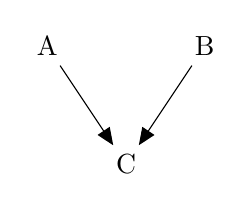
\begin{tikzpicture}
  \node (A) at (0,0) {A};
  \node (B) at (2,0) {B};
  \node (C) at (1,-1.5) {C};
  \draw[->] (A) -- (C);
  \draw[->] (B) -- (C);
  \end{tikzpicture}


  Type 2:
  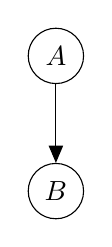
\begin{tikzpicture}
  \node[latent] (A) {$A$};
  \node[latent, below = of A] (B) {$B$};
  \edge {A} {B};
  \end{tikzpicture}
  \iffalse
  \fi
  
 
  \subsection{Use pagckages: adigraph}

  \NewAdigraph{myAdigraph}{
    s:0,0;
    1:2,2;
    3:2,-2;
    2:6,2;
    4:6,-2;
    t:8,0;
}{
    s,1:25;
    s,3:25;
    3,4:25;
    1,2:35;
    2,t:20;
    4,t:30;
    3,1:10;
    4,2:10;
    2,3:15::near start;
    4,1:5::near start;
}
\myAdigraph{}

\newpage


% --------------------------------------
\section{Using packages}
Packages are like plugins to extend the Latex' capabilities. Some common commands are listed here.

\begin{lstlisting}[language=bash, caption={tlmgr commands and etc}]
tlmgr list --only-installed   # show installed packages

tlmgr search <package-name>   # search a packages
tlmgr info <package-name>     # show a package's intro, no matter installed or not
tlmgr install <package-name>  # install a new packages

tlmgr update --self --all     # update package index

kpsewhich article.sty         # locate a package's .sty file

# env variables can define additional directories to be searched. 
echo $TEXMFHOME $TEXMFLOCAL $TEXMFSYSCONFIG 
\end{lstlisting}
\newpage


% --------------------------------------
\section{Generate Slides}
Use the package beamer to generate a pdf file of slides from an article


\begin{lstlisting}[caption={Changes in .tex file}]
  % \documentclass{article}
  \documentclass{beamer}
  \usetheme{Madrid}
\end{lstlisting}

% --------------------------------------
\end{document}
  \newpage
  \documentclass{article}
% \documentclass{beamer}
% \usetheme{Madrid}

%------------------------------
% used for href/url
\usepackage{hyperref}


% used for math fomulas
\usepackage{amsmath}

% used for pictures
\usepackage{graphicx}
\usepackage{subcaption}
\usepackage{float}

% used for codes
\usepackage{listings}
\lstset{
  basicstyle=\ttfamily\footnotesize, % Set your code to be drawn with a monospaced font
  breaklines=true, % Enables line breaking
  frame=single % Adds a frame around the code
}

% used for Graph
\usepackage{adigraph}

% used for Bayesian Network
\usepackage{tikz}
\usetikzlibrary{bayesnet}

%------------------------------
% TODO 
\tolerance=10000
\emergencystretch=\maxdimen
\hyphenpenalty=10000
\hbadness=10000


\usepackage{silence}
\WarningFilter{latex}{Overfull \hbox}

%------------------------------



\title{MK's Notes for CIVL-4530 Geometric Design}
\date{2024-03-04}
\author{Michael Chen}

\begin{document}
  % \pagenumbering{gobble}
  % \maketitle
  % \newpage
  % \pagenumbering{arabic}
  \setcounter{section}{1}


  % todo ----------------------------------------
  % \tableofcontents
  % \newpage


  % ----------------------------------------
  \section{Design Control and Criteria}
  \subsection{Objectives}
  \begin{enumerate}
    \item Design Vehicles, Driver and Traffic Characteristics
    \item 13 AASHTO criteria
    \item AASHTO administered, federal-wide
    \item State-DOT administered - Green Book
    \item local goverment administered - ordinance or code
  \end{enumerate}

  \subsection{Design vehicles}
  \begin{enumerate}
    \item Design Vehicle\\ 
    Its weight, dimensions, and operating characteristics will be used to establish the geometric standards of the highway.
    \item design vehicle P: passenger car
    \begin{enumerate}
      \item Geometry - length 19ft (5+11+3), width 7ft
      \item Minimum turning path - outline 25.4ft, front wheel 23.8ft, CTR 21ft, min 14.4ft 
    \end{enumerate}
    \item WB-50 - length 55ft, width 8.5ft, height 13.5ft
  \end{enumerate}

  ASSHTO guideline - Selection of design vehicle \ref{fig:image-design-vehicles}
  \begin{figure}[!ht]
    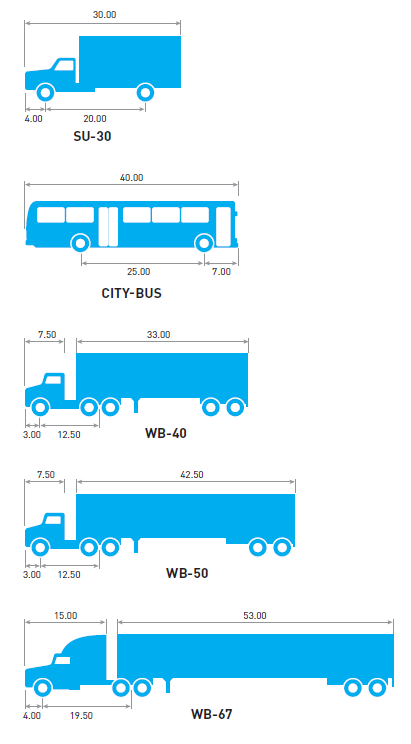
\includegraphics[width=0.7\linewidth]{design-vehicles.png}
    \caption{Design Vehicles}
    \label{fig:image-design-vehicles}
  \end{figure}
  \begin{enumerate}
    \item parking lot - passenger car
    \item intersection of local area - SU-30, 30ft
    \item intersection of state highway and city street - City transit buses, 40ft
    \item intersections of highways; low-volume county roads with ADT < 400 - City bus (40ft, 84 passengers) or conventional bus(36ft, 64 passengers)
    \item freeway ramp; arterial crossroads; intersections of state highways; with high volume of traffic - WB-40 to WB-62
  \end{enumerate}

  \subsection{Older Driver Deficiencies}
  \begin{enumerate}
    \item Slower information processing
    \item Slower reaction times
    \item Slower decision making
    \item Visual deterioration
    \item Hearing deterioration
    \item Decline in ability to judge time, speed, and distance
    \item Limited depth perception
    \item Limited physical mobility
    \item Side effects from prescription drugs
  \end{enumerate}

  \subsection{LOS and ADT}
  acceptable LOS / level of "congestion" \ref*{fig:image-LOS} \\

  \begin{tabular}{|c|c|c|c|c|}
    Roadway & urban & rural level & rural rolling & rural mountainous\\
    \hline
    Freeway & C/D   & B & B & C\\
    Arterial & C/D  & B & B & C\\
    Collector & D   & C & C & D\\
    Local & D       & D & D & D\\
  \end{tabular}
  \begin{figure}[h!]
    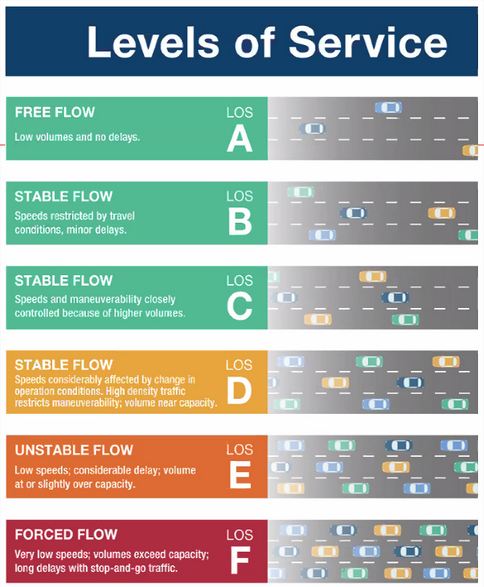
\includegraphics[width=\linewidth]{LOS.png}
    \caption{Level of Service}
    \label{fig:image-LOS}
  \end{figure}

  \subsection{13 AASHTO Criteria}
  \begin{enumerate}
      \item design speed
      \item lane width
      \item shoulder width
      \item bridge width
      \item structural capacity
      \item 
      \item horizontal alignment
      \item vertical alignment
      \item cross slope
      \item grades
      \item superelevation
      \item horizontal clearance
      \item vertical clearance
  \end{enumerate}

  \subsection{speed}
  \begin{enumerate}
    \item running speed - the speed of an individual vehicle
    \item design speed - AASHTO: max safe speed
    \item operation speed - the 85th percentile of observed speed in free flow conditions
    \item safty of over speed - $\Delta$V: [0, 5] low; [5, 15] medium; [15, infinit] high
  \end{enumerate}

  minimum design speed for \textbf{rural} roadways vs vehicle per day(VPD)
  \begin{tabular}{|c|c|c|c|}
    \hline
    rural terrain & 0-400 & 400-2000 & over 2000 \\
    \hline
    level         & 40    & 50       & 60 \\
    rolling       & 30    & 40       & 50 \\
    mountainous   & 20    & 30       & 40 \\
  \end{tabular}

  \subsection{lane width for urban and rural (1-2ft wider than urban)}
  \begin{tabular}{|l|l|l|}
    Types & urban & rural \\
    \hline
    Freeway and Interstates: & 12ft, & 12ft\\
    Ramp: & 12-30ft & 12-30ft \\ 
    Arterial: & 11-12ft, & 10-12ft \\
    Collections: & 10-12ft, & 10-12ft\\
    local roads: & 9-12ft, & 9-12ft  \\
  \end{tabular}

  \subsection{cross slope}
  paved surfaces: 1.5-2\%, typical 2\%  - Green Book\\
  unpaved surfaces: 2-6\% - Green Book\\
  areas with high intensity rainfall: 2-2.5\% \\
  ALDOT use in 2 Counties: 2.2\% \\



\begin{table}[ht]
\centering
\caption{Lane Widths for Different Types of Roadways}
\label{tab:lane_widths}
\begin{tabular}{@{}lcccc@{}}
\hline
\textbf{Type of Roadway} & \multicolumn{2}{c}{\textbf{Rural}} & \multicolumn{2}{c}{\textbf{Urban}} \\
                         & \textbf{US (feet)} & \textbf{Metric (meters)} & \textbf{US (feet)} & \textbf{Metric (meters)} \\ 
\hline
Freeway                  & 14-16*             & 4.3-4.9*                & 14–16*             & 4.3–4.9*                \\
Arterial                 & 14-16              & 4.3-4.9                 & 14–16              & 4.3–4.9                 \\
Collector                & 14                 & 4.3                     & 14                 & 4.3                     \\
Local                    & 14                 & 4.3                     & 14                 & 4.3                     \\
\hline
\end{tabular}
\end{table}




\begin{table}[ht]
\centering
\caption{Functional Classification of Roadways}
\label{tab:functional_classification}
\begin{tabular}{@{}lccc@{}}
\hline
\textbf{Criteria} & \textbf{Local} & \textbf{Collector} & \textbf{Arterial} \\
\hline
Street pavement width & 24 ft & 22 ft (1), 31 ft & 36 ft (2), 48 ft \\
Minimum horizontal curve radius & 200 ft & 350 ft & 550 ft \\
Maximum grade (3) & 15\% & 12\% & 8\% \\
Minimum design speed for vertical curve & 25 mi/h & 35 mi/h & 45 mi/h \\
\hline
\end{tabular}
\end{table}


  % ----------------------------------------
  \subsection{Terms}
  SU - represents all single unit trucks and small buses, with length 35-60ft \\
  ADT - average daily traffic \\
  AADT - the annual average daily traffic, empersizing annual average \\
  DHV - design hour volume \\
  DDHV - The directional design hour volume \\
  30HV - the 30th Highest Hour of Yearly Traffic - the 30th Hour volume \\
  design speed (DS) - design maximum speed of a roadway \\
  free flow speed (FFS) - the observed speed at which vehicles can travel with minimal delays and no restrictions from traffic signals, congestion, or other factors. \\
  LOS - Characterization of operating conditions, related to speed, travel time, traffic density, freedom to maneuver  \\
  FFS is close to DS - It means a good design \\
  K-factor - DHV = K * ADT, K is 8 to 12\% for urban facilities; 12 to 18\% for rural facilities.  \\
  D-factor - DDHV = D * DHV, D is 50\% for urban highways; 55 - 80\% for rural and suburban roads \\
  DDHV = ADT (or AADT) * K * D \\
  CMF - Crash Modification Factor \\
  Cul-de-sac: deed end street \\

  \subsection{Rules}
  Tandem Axle - 2 axles which are very close\\
  State maximum gross vehicle weight - 73,280 - 164,000 lbs\\
  State maximum gross vehicle weight - 73,280 - 164,000 lbs\\
  \\
  DHV = 8\% - 12\% ADT in urban area, refer to Green Book\\
  30HV = 15\% ADT in a typical rural arterial, refer to Green Book\\

  % ----------------------------------------
  \subsection{Formulas}
  1 mile = 5,280 feet \\
  1000 kg = 2204.62 lbs \\
  1 foot = 0.3048 meters \\
  1 lb = 16 oz \\
  1 gallon = 3.785 liters (U.S. liquid gallon) \\
  1 gallon = 4.546 liters (U.K. imperial gallon) \\


  % ----------------------------------------
  \subsection{Reference}
  FHWA Website \\
  http://safety.fhwa.dot.gov/geometric/pubs/mitigationstrategies/ \\



\end{document}

  \newpage
  \documentclass{article}
% \documentclass{beamer}
% \usetheme{Madrid}

%------------------------------
% used for href/url
\usepackage{hyperref}


% used for math fomulas
\usepackage{amsmath}

% used for tables
\usepackage{booktabs} % For better looking tables

% used for pictures
\usepackage{graphicx}
\usepackage{subcaption}
\usepackage{float}

% used for codes
\usepackage{listings}
\lstset{
  basicstyle=\ttfamily\footnotesize, % Set your code to be drawn with a monospaced font
  breaklines=true, % Enables line breaking
  frame=single % Adds a frame around the code
}

% used for Graph
\usepackage{adigraph}

% used for Bayesian Network
\usepackage{tikz}
\usetikzlibrary{bayesnet}

%------------------------------
% TODO 
\tolerance=10000
\emergencystretch=\maxdimen
\hyphenpenalty=10000
\hbadness=10000


\usepackage{silence}
\WarningFilter{latex}{Overfull \hbox}

%------------------------------



\title{MK's Notes for CIVL-4530 Geometric Design}
\date{2024-03-04}
\author{Michael Chen}

\begin{document}
  \pagenumbering{gobble}
  % \maketitle      % hide title page
  % \newpage
  \pagenumbering{arabic}
  \setcounter{page}{30}   % start from page 30
  % \pagenumbering{roman}


  % ----------------------------------------
  \tableofcontents
  \newpage


  % ----------------------------------------
  % Geometric Design is a basic course of Transportation, introducing principal concepts and fomulas.
  % \newpage

  % ----------------------------------------
  \setcounter{section}{2}
  \section{Chapter 03 Sight Distance (SD)}
  \subsection{Objectives}
  \begin{enumerate}
    \item describe various types of sight distance
    \item determine sight distance requirements for stopping and passing maneuvers
  \end{enumerate}

  \subsection{key component of SD}
  \begin{enumerate}
    \item PRT: the perception-reaction time required to initiate a maneuver (pre-maneuver phase)
    \item MT: the time requried to safely complete a maneuver
  \end{enumerate}
  driver's eye - 3.5ft high\\
  Hazard - 2ft high \\


  \subsection{Sight Distance Types}
  \begin{enumerate}
    \item stopping sight distance (SSD)
    \item decision sight distance (DSD)
    \item passing sight distance (PSD)
    \item intersection sight distance (ISD)
  \end{enumerate}

  \subsection{SSD - stopping sight distance}
  SSD is a key input for geometric design, including horizontal and vertical alignment \\
  \\
  PRT includes: recognize an object + decide a stop + react and prepare to apply the brake \\
  Deceleration rate: $11.2ft/sec^{2}$, 10th percentile deceleration rate, by AASHTO \\
  \begin{align*}
    SSD & = D_{p-r} + D_{b}\\
        & \textbf{$D_{p-r}$: in ft, perception-reaction distance} \\
        & \textbf{$D_{b}$: in ft, braking distance} \\
        \\
    D_{p-r} & = 1.47 \times 2.5s \times v = 3.675v \\
            & \textbf{$D_{p-r}$: in ft, perception-reaction distance} \\
            & \textbf{v: in mi/h, design speed} \\
            \\
    D_{b} & = \frac{(v_{0})^2 - (v_{f})^2}{30(\frac{a}{g} \pm G)} \\
          & \textbf{$D_{b}$: in ft, braking distance}\\
          & \textbf{$v_{0}$: in mi/h, design speed} \\
          & \textbf{$v_{f}$: in mi/h, final velocity}\\
          & \textbf{a: 11.2 $ft/sec^2$, deceleration rate, by AASHTO, in [10, 15]} \\
          & \textbf{g: 32.2 $ft/sec^2$} \\
          & \textbf{f = a/g: 0.35 by ASSHTO, coefficient of friction, 0.7 for dry roads, 0.3-0.4 for wed roads} \\
          & \textbf{G: grade, e.g. down grade: -0.06} \\
  \end{align*}

  \subsection{SSD on vertical curve}
  crest curve: \\
    - Driver eye height: 3.5ft \\
    - Height of object in readway: 2.0ft \\
    \\
  sag curve: \\
    - headlight height: 2ft \\
    - headlight beam angle: 1 degree (departure from horizontal, suggest changing to 0.75 degree)


  \subsection{DSS - decision sight distance}
  For A or B (avoidance maneuvers): \\
  $DSD = 1.47V_{t} + 1.075(V^2/a)$ \\
  \\
  For C, D, and E: \\
  $DSD = 1.47V_{t}$ \\
  \\

  \subsection{DSS - decision sight distance}
  Decision sight distance for various conditions: \\
  \\
  Avoidance Maneuver A: Stop on rural road, t = 3.0 s\\
  Avoidance Maneuver B: Stop on urban road, t = 9.1 s\\
  \\
  Avoidance Maneuver C: Speed/path/direction change on rural road, t varies between 10.2 and 11.2 s \\
  Avoidance Maneuver D: Speed/path/direction change on suburban road, t varies between 12.1 and 12.9 s \\
  Avoidance Maneuver E: Speed/path/direction change on urban road, t varies between 14.0 and 14.5 s \\
  \\
  Source: AASHTO Green Book, 2011, Table 3-3\\



  \begin{table}[h!]
  \centering
  \caption{U.S. Customary Decision Sight Distance}
  \label{tab:us_customary_decision_sight_distance}
  \begin{tabular}{ccccccc}
  \toprule
  Design Speed (mph) & \multicolumn{5}{c}{Decision Sight Distance (ft)} &  \\
  \cmidrule(lr){2-6}
  & A & B & C & D & E & \\
  \midrule
  30 & 220 & 490 & 450 & 535 & 620 & \\
  35 & 275 & 590 & 525 & 625 & 720 & \\
  40 & 330 & 690 & 600 & 715 & 825 & \\
  45 & 395 & 800 & 675 & 800 & 930 & \\
  50 & 465 & 910 & 750 & 890 & 1030 & \\
  55 & 535 & 1030 & 865 & 980 & 1135 & \\
  60 & 610 & 1150 & 990 & 1125 & 1280 & \\
  65 & 695 & 1275 & 1050 & 1220 & 1365 & \\
  70 & 780 & 1410 & 1105 & 1275 & 1445 & \\
  75 & 875 & 1545 & 1180 & 1365 & 1545 & \\
  80 & 970 & 1685 & 1260 & 1455 & 1650 & \\
  \bottomrule
  \end{tabular}
  \end{table}

  \begin{table}[h!]
  \centering
  \caption{Metric Decision Sight Distance}
  \label{tab:metric_decision_sight_distance}
  \begin{tabular}{ccccccc}
  \toprule
  Design Speed (km/h) & \multicolumn{5}{c}{DSD (m)} \\
  \cmidrule(lr){2-6}
  & A & B & C & D & E \\
  \midrule
  50 & 70 & 155 & 145 & 170 & 195 \\
  60 & 95 & 195 & 170 & 205 & 235 \\
  70 & 115 & 325 & 200 & 235 & 275 \\
  80 & 140 & 280 & 230 & 270 & 315 \\
  90 & 170 & 325 & 270 & 315 & 360 \\
  100 & 200 & 370 & 315 & 355 & 400 \\
  110 & 235 & 420 & 330 & 380 & 430 \\
  120 & 265 & 470 & 360 & 415 & 470 \\
  130 & 305 & 525 & 390 & 450 & 510 \\
  \bottomrule
  \end{tabular}
  \end{table}

  \newpage

  \subsection{PSD - Passing sight distance}
  passing vehicle speed - passed vehicle speed $>=$ 12 mi/h\\
  \\
  On two-lane rural highways\\
  overtaking and returning to lane\\
  before opposing vehicle reaches passing vehicle\\


  \subsection{Passing sight distance assumptions - Green Book}
  \begin{enumerate}
    \item Speeds of passing and opposing vehicles equal the design speed
    \item Speed differential between the passing and passed vehicle is 12 mi/h
    \item Design vehicle is passenger car for all vehicles involved
    \item Perception-reaction time to decide to abort is 1 second
    \item Deceleration rate in abort maneuver is $11.2 ft/sec^2$
    \item Headway at end of maneuver is 1 second
  \end{enumerate}



  \begin{table}
  \centering
  \caption{U.S. Customary Assumed Speeds and Passing Sight Distance}
  \label{tab:us_customary_speeds}
  \begin{tabular}{cccc}
  \toprule
  Design Speed (mph) & Passed Vehicle (mph) & Passing Vehicle (mph) & Passing Sight Distance (ft) \\
  \midrule
  20 & 8  & 20 & 400 \\
  25 & 13 & 25 & 450 \\
  30 & 18 & 30 & 500 \\
  35 & 23 & 35 & 550 \\
  40 & 28 & 40 & 600 \\
  45 & 33 & 45 & 700 \\
  50 & 38 & 50 & 800 \\
  55 & 43 & 55 & 900 \\
  60 & 48 & 60 & 1000 \\
  65 & 53 & 65 & 1100 \\
  70 & 58 & 70 & 1200 \\
  75 & 63 & 75 & 1300 \\
  80 & 68 & 80 & 1400 \\
  \bottomrule
  \end{tabular}
  \end{table}
  
  \begin{table}[h!]
  \centering
  \caption{Metric Passing Sight Distance}
  \label{tab:metric_passing_sight_distance}
  \begin{tabular}{cccc}
  \toprule
  Design Speed (km/h) & Assumed Speeds Passed Vehicle (km/h) & Passing Vehicle (km/h) & PSD (m) \\
  \midrule
  30 & 11 & 30 & 120 \\
  40 & 21 & 40 & 140 \\
  50 & 31 & 50 & 160 \\
  60 & 41 & 60 & 180 \\
  70 & 51 & 70 & 210 \\
  80 & 61 & 80 & 245 \\
  90 & 71 & 90 & 280 \\
  100 & 81 & 100 & 320 \\
  110 & 91 & 110 & 355 \\
  120 & 101 & 120 & 395 \\
  130 & 111 & 130 & 440 \\
  \bottomrule
  \end{tabular}
  \end{table}
  
  


  % todo ----------------------------------------



  \subsection{vertical sight distance - Sighting Rod and Target Rod - AASHTO}
  Sighting rod (driver eye, used by observer):  3.5ft tall \\
  \\
  Target rod (object, used by assistant): 4.25ft tall
  \\


  \subsection{ISD - Intersection Sight Distance}
  \begin{enumerate}
    \item \textbf{a.k.a Green Book/PGDHS:} A Policy on Geometric Design of Highways and Streets, 2018, 7th Edition
    \item Guidelines for Geometric Design of Very Low Volume Local Roads, 2001
    \item A Guide to Achieving Flexibility in Highway Design, May 2004
    \item Guide for the Planning, Design, and Operation of Pedestrian Facilities, July 2004
    \item Guide for the Development of Bicycle Facilities, June 2012

    \item Good for New Highway Design 
    \item TRB Special Report 214, Designing Safer Roads: Practices for Resurfacing, Restoration, and Rehabilitation for guidance. \\
  \end{enumerate}

  

  \subsection{ISD - formula}
  The Intersection Sight Distance (ISD) is given by the formula:
  \begin{equation}
      ISD = 1.47 V_{\text{major}} \times t_g
  \end{equation}
  where:
  \begin{itemize}
      \item $ISD$ in ft, the intersection sight distance (length of the leg of sight triangle along the major road)
      \item $V_{\text{major}}$ in mph, the design speed of the major road in miles per hour (mph).
      \item $t_g$ in seconds, is the time gap for a minor road vehicle to enter the major road
  \end{itemize}
  where $t_g$:
  \begin{itemize}
      \item design vehicle: passenger car 7.5s; single-unit truck 9.5s; combination truck 11.5s
      \item a stopped vehicle turns \textbf{left} to a 2-lane highway; without median; grade $<= 3\%$
      \item Major highway: each additional lane, passenger car $+ 0.5s$; trunck $+ 0.7s$;
      \item Minor road: grade $> 3\%$, add 0.3s for each percent grade
  \end{itemize}






  \subsection{design elements}
  Design elements affect design consistency, driver expectancy, and vehicular operation.
  \begin{enumerate}
    \item horizontal and vertical alignment
    \item embankments and slopes
    \item shoulders, crown and cross slope, superelevation
    \item bridge widths
    \item signing and delineation
    \item guardrail and placement of utility poles or light supports
  \end{enumerate}

  \subsection{Highway Design Control Factors}
  \begin{enumerate}
    \item Highway Function (Arterials, Collections, Locals)
    \item Design speed of the facility
    \item Physical characteristics of the "design vehicle" 
    \item Performance of the design vehicle (heavy trucks, RVs)
    \item Acceptable degree of congestion
  \end{enumerate}

  \subsection{Highway functions}
    Highway Function: Arterials, Collections, Locals \\
    Arterials: principal arterials, minor arterials
    Mobility: the ability to move goods and passengers to their destination in a reasonable time 
    Accessibility: the ability to reach desired destination

  \subsection{Hierarchy of Movements - 6 stages}
  Main Movement \\
  Transition \\
  Distribution \\
  Collection \\
  Access \\
  Termination \\

  \subsection{Hierarchy of Movements}
	\begin{tabular}{|l|p{2cm}|p{2cm}|p{2cm}|p{2cm}|p{2cm}|}
	\hline
	\textbf{Roadway Class} & \textbf{\% Through Movement} & \textbf{VMT in Rural} & \textbf{Miles in Rural} & \textbf{VMT in Urban} & \textbf{Miles in Urban} \\
	\hline
	Freeways      & 100\%     &     &  \\
	Arterials     & 60-80\%   & {\bfseries 45-75\%} & 6-12\%  & {\bfseries 65-80\%}   & 15-25\% \\
	Collectors    & 40-60\%   & 20-35\% & 20-25\% & 5-19\%    & 5-10\% \\
	Local Streets & 0-40\%    & 5-20\%  & {\bfseries 65-75\%} & 10-30\%   & {\bfseries 65-80\%} \\
	\hline
	\end{tabular}

  \subsection{Highway Design Volume}
  \begin{tabular}{|l|l|l|}
  \hline
  Highway Type & Approximate Design Speed & Approximate Design Volume \\
  \hline
  Freeway – free flow & 70-75 mph & 2400 veh/h/ln \\
  Freeway – free flow & 65 mph & 2300 veh/h/ln \\
  \hline
  Rural Highways & & \\
  a) Multilane-one way & & 1600-2000 veh/h/ln \\
  b) Two lane & & 2000-2800 veh/h \\
  \hline
  Urban Highways & & \\
  a) Arterials & & See Highway Capacity Manual \\
  b) Signalized intersections & & 1900 pc/h/ln \\
  c) Unsignalized intersections & & 1100-2000 veh/h \\
  \hline
  \end{tabular}

  \subsection{Traffic Information for Roadway Designers}
  These traffic information should be available to the designer prior to or very early in the design process:
  \begin{enumerate}
    \item AADT for the current year: opening year (completion of construction), and design year
    \item Existing hourly traffic volumes over a minimum of 24-hour period, including peak hour turning movements and pedestrian counts
    \item Directional distribution factor (D30).
    \item 30th highest hour factor (K30).
    \item Truck factors (T) for daily and peak hour.
    \item Design speed and proposed posted speed.
    \item Design vehicle for geometric design.
    \item Turning movements and diagrams for existing and proposed signalized intersections.
    \item Special or unique traffic conditions, including during construction.
    \item Crash history, including analyses at high crash locations within the project limits.
    \item Recommendations regarding parking or other traffic restrictions.
  \end{enumerate}




  % ----------------------------------------
  \subsection{Terms}
  \begin{enumerate}
    \item PRT - perception-reaction time
    \item MT - maneuver time
    \item trajectory -  
    \item 
  \end{enumerate}


  \subsection{Rules}

  % ----------------------------------------
  \subsection{Formulas}

  % ----------------------------------------

  \subsection{Reference}

  \newpage





% --------------------------------------
\end{document}
  \newpage
  \documentclass{article}
% \documentclass{beamer}
% \usetheme{Madrid}

%------------------------------
% used for href/url
\usepackage{hyperref}


% used for math fomulas
\usepackage{amsmath}

% used for pictures
\usepackage{graphicx}
\usepackage{subcaption}
\usepackage{float}

% used for codes
\usepackage{listings}
\lstset{
  basicstyle=\ttfamily\footnotesize, % Set your code to be drawn with a monospaced font
  breaklines=true, % Enables line breaking
  frame=single % Adds a frame around the code
}

% used for Graph
\usepackage{adigraph}

% used for Bayesian Network
\usepackage{tikz}
\usetikzlibrary{bayesnet}

%------------------------------
% TODO 
\tolerance=10000
\emergencystretch=\maxdimen
\hyphenpenalty=10000
\hbadness=10000


\usepackage{silence}
\WarningFilter{latex}{Overfull \hbox}

%------------------------------



\title{MK's Notes for CIVL-4530 Geometric Design}
\date{2024-03-04}
\author{Michael Chen}

\begin{document}
  \pagenumbering{gobble}
  % \maketitle
  % \newpage
  \pagenumbering{arabic}
  \setcounter{page}{40}


  % ----------------------------------------
  \tableofcontents
  \newpage


  % ----------------------------------------
  \setcounter{section}{3}
  \section{Chapter 04 horizontal Alignment}
  \subsection{Objectives}
  \begin{enumerate}
    \item Horizontal Curve Elements
    \item Superelevation
    \item Design Horizontal Curve
  \end{enumerate}

  \subsection{D - degree of curvature}
  \begin{enumerate}
    \item D: in degree
    \item highways:(small) D $->$ arc length of 100ft
    \item railroads(big) D $->$ cord length of 100ft
    \item Relationship btw D and R -> $D / 100 = 360 / 2\pi R$
  \end{enumerate}

  

  \subsection{Horizontal Curve}
  Terms:
  \begin{enumerate}
    \item PC: intersection of tangent and curve
    \item PT: intersection of tangent and curve
    \item PI: intersection of 2 tangents
    \item PCurve: intersection of line PI-O and curve PC-PT
    \item PChord: intersection of chord PC-PT and line PI-O
    \item 
    \item R: the radius of the curve
    \item D: in degree, the degree matches 100ft arc
    \item $\Delta$ - the degree for the curve
    \item 
    \item L: in feet, curve length 
    \item T: in feet/meter, line segment from PI to PT/PC
    \item 
    \item E: line segment of PI-PCurve
    \item M: line segment of PCurve-PChord 
    \item LC: chord PC-PT 
    \item 
    \item curvature - how big is a curve, $curvature = 1/R$
  \end{enumerate}
  Formulas:
  \begin{align*}
     \frac{D}{100} & = \frac{360}{2\pi R} \\
     D & = \frac{360 \cdot 100}{2\pi R} \\
     L & = 100 \cdot \Delta / D \\
     L_{in\_meter} & = 30.48 \cdot \Delta / D \\
     T & = R \cdot tan \frac{1}{2}\Delta \\
     M & = R(1-cos \frac{1}{2} \Delta) \\
     E & = R(\frac{1}{cos \frac{1}{2} \Delta} - 1) \\
     LC & = 2R \cdot sin \frac{1}{2} \Delta \\
  \end{align*}

  % TODO
  \begin{enumerate}
    \item make criteria matches  
    \begin{enumerate}
      \item driver expectancy/behavior
      \item vehicle performance/behavior
    \end{enumerate}
    \item balance safty, cost, mobility, community values, environmental, politics, liability, sustainable development, etc
  \end{enumerate}

  \subsection{AASHTO Role}
  \begin{enumerate}
    \item American Association of State Highway and Transportation Officials
    \item the membership of AASHTO consists of FHWA, and state DOTs
  \end{enumerate}

  % ----------------------------------------
  \subsection{Reference - AASHTO publications}
  \begin{enumerate}
    \item \textbf{a.k.a Green Book/PGDHS:} A Policy on Geometric Design of Highways and Streets, 2018, 7th Edition
    \item Guidelines for Geometric Design of Very Low Volume Local Roads, 2001
    \item A Guide to Achieving Flexibility in Highway Design, May 2004
    \item Guide for the Planning, Design, and Operation of Pedestrian Facilities, July 2004
    \item Guide for the Development of Bicycle Facilities, June 2012

    \item Good for New Highway Design 
    \item TRB Special Report 214, Designing Safer Roads: Practices for Resurfacing, Restoration, and Rehabilitation for guidance. \\
  \end{enumerate}

  \subsection{Reference - ITE publications}
  ITE - Institute of Transportation Engineers. It is an international educational and scientific association of transportation professionals.\\
  \begin{enumerate}
    \item Urban Street Geometric Design Handbook, 2008
    \item Freeway and Interchange Geometric Design Handbook, 2007
    \item Designing Walkable Urban Thoroughfares: A Context Sensitive Approach, March 2010
  \end{enumerate}

  \subsection{design elements}
  Design elements affect design consistency, driver expectancy, and vehicular operation.
  \begin{enumerate}
    \item horizontal and vertical alignment
    \item embankments and slopes
    \item shoulders, crown and cross slope, superelevation
    \item bridge widths
    \item signing and delineation
    \item guardrail and placement of utility poles or light supports
  \end{enumerate}

  \subsection{Highway Design Control Factors}
  \begin{enumerate}
    \item Highway Function (Arterials, Collections, Locals)
    \item Design speed of the facility
    \item Physical characteristics of the "design vehicle" 
    \item Performance of the design vehicle (heavy trucks, RVs)
    \item Acceptable degree of congestion
  \end{enumerate}

  \subsection{Highway functions}
    Highway Function: Arterials, Collections, Locals \\
    Arterials: principal arterials, minor arterials
    Mobility: the ability to move goods and passengers to their destination in a reasonable time 
    Accessibility: the ability to reach desired destination

  \subsection{Hierarchy of Movements - 6 stages}
  Main Movement \\
  Transition \\
  Distribution \\
  Collection \\
  Access \\
  Termination \\

  \subsection{Hierarchy of Movements}
	\begin{tabular}{|l|p{2cm}|p{2cm}|p{2cm}|p{2cm}|p{2cm}|}
	\hline
	\textbf{Roadway Class} & \textbf{\% Through Movement} & \textbf{VMT in Rural} & \textbf{Miles in Rural} & \textbf{VMT in Urban} & \textbf{Miles in Urban} \\
	\hline
	Freeways      & 100\%     &     &  \\
	Arterials     & 60-80\%   & {\bfseries 45-75\%} & 6-12\%  & {\bfseries 65-80\%}   & 15-25\% \\
	Collectors    & 40-60\%   & 20-35\% & 20-25\% & 5-19\%    & 5-10\% \\
	Local Streets & 0-40\%    & 5-20\%  & {\bfseries 65-75\%} & 10-30\%   & {\bfseries 65-80\%} \\
	\hline
	\end{tabular}

  \subsection{Highway Design Volume}
  \begin{tabular}{|l|l|l|}
  \hline
  Highway Type & Approximate Design Speed & Approximate Design Volume \\
  \hline
  Freeway – free flow & 70-75 mph & 2400 veh/h/ln \\
  Freeway – free flow & 65 mph & 2300 veh/h/ln \\
  \hline
  Rural Highways & & \\
  a) Multilane-one way & & 1600-2000 veh/h/ln \\
  b) Two lane & & 2000-2800 veh/h \\
  \hline
  Urban Highways & & \\
  a) Arterials & & See Highway Capacity Manual \\
  b) Signalized intersections & & 1900 pc/h/ln \\
  c) Unsignalized intersections & & 1100-2000 veh/h \\
  \hline
  \end{tabular}

  \subsection{Traffic Information for Roadway Designers}
  These traffic information should be available to the designer prior to or very early in the design process:
  \begin{enumerate}
    \item AADT for the current year: opening year (completion of construction), and design year
    \item Existing hourly traffic volumes over a minimum of 24-hour period, including peak hour turning movements and pedestrian counts
    \item Directional distribution factor (D30).
    \item 30th highest hour factor (K30).
    \item Truck factors (T) for daily and peak hour.
    \item Design speed and proposed posted speed.
    \item Design vehicle for geometric design.
    \item Turning movements and diagrams for existing and proposed signalized intersections.
    \item Special or unique traffic conditions, including during construction.
    \item Crash history, including analyses at high crash locations within the project limits.
    \item Recommendations regarding parking or other traffic restrictions.
  \end{enumerate}




  % ----------------------------------------
  \subsection{Terms}
  \begin{enumerate}
    \item cross section - A cross section refers to the vertical view of a roadway or highway at right angles to its centerline. 
    \item embankment - An embankment is a constructed mound of earth, stones, or other materials. Its purpose is to support the raising of a roadway or railway above the level of the surrounding ground surface.
    \item cross slope - Cross slope plays a crucial role in ensuring proper drainage and safety on roadways.
    \item crown - The crown of a highway refers to the cross-sectional shape of the road surface.
    \item signing and delineation -  
    \item guardrail - A guardrail on a highway serves as a safety barrier designed to protect motorists.
    \item guardrail and placement of utility poles or light supports - 
    \item  detour - walkaround roadway  
    \item through movement - refers to the uninterrupted flow of vehicles or goods from one location to another 
    \item VMT - Vehicle Miles Traveled
    \item open year and design year - open year means compeletion of construction. 
    \item $D_{30}$ factor - Directional Distribution factor 
    \item $K_{30}$ factor - the 30th highest hour factor 
  \end{enumerate}


  \subsection{Rules}

  % ----------------------------------------
  \subsection{Formulas}

  % ----------------------------------------

  \subsection{Reference}

  \newpage





% --------------------------------------
\end{document}
  \newpage



% --------------------------------------
\end{document}